\section{Activity Selection}\label{greedy: sec: activity selection}\doHeader{Activity Selection}

Here is another example where the algorithm makes one greedy choice, then recurses.
 
\paragraph{Problem definition.}
The (unweighted) \prob{Activity Selection} problem is defined as follows:

\begin{mylist}
\item[\bf input:]
  A collection of real intervals $I=([s_1, e_1], [s_2, e_2], …, [s_n, e_n])$,
  with $s_j \le e_j$ for all $j$.
  % [review 2026-09-27] fix: endpoint was written $t_j$ but the intervals are $[s_j, e_j]$; changed to $e_j$
  We use $J_j$ to denote $[s_j,e_j]$, and call $J_j$ a \emph{job}.
  We think of $[s_j, e_j]$ as the time interval the job requires.

\item[\bf output:]
  A maximum-size pairwise-disjoint subset $S$ of $I$.
\end{mylist}

\emph{Pairwise disjoint} means that every two intervals in $S$ are disjoint
(that is, for every two intervals, their intersection is empty).
Intuitively,
we want to do as many jobs as we can,
but for any two jobs whose intervals overlap, we can't do both.
To build intuition, consider an example:

\smallskip

\centerline{
  \begin{tikzpicture}[scale=0.5]\footnotesize
  \draw (5,0) -- ++(-2,0) node[anchor=south] {$J_1$} -- ++(-2,0); 
  \draw (7,1) -- ++(-2,0) node[anchor=south] {$J_2$} -- ++(-2,0); 
  \draw (8,0) -- ++(-1,0) node[anchor=south] {$J_3$} -- ++(-1,0); 
  \draw (10,3) -- ++(-3,0) node[anchor=south] {$J_4$} -- ++(-2.5,0); 
  \draw (12,2) -- ++(-2.75,0) node[anchor=south] {$J_5$} -- ++(-2.75,0); 
  \draw (13,0) -- ++(-2,0) node[anchor=south] {$J_6$} -- ++(-2,0); 
  \draw (14,1) -- ++(-1.5,0) node[anchor=south] {$J_7$} -- ++(-1.5,0); 
\end{tikzpicture}
}

\smallskip

One correct solution for this input is $S^*= \{J_1, J_3, J_6\}$.

The goal is to maximize the size $|S^*|$ of $S^*$.
Note that the size is the \emph{number of intervals} in $S$,
not the total area covered by intervals in $S$.

\paragraph{Coming up with an algorithm.}

A greedy algorithm for this problem should maintain a subset $X\subseteq I$ of the jobs.
It should start with $X$ empty, then add jobs one by one,
until no more jobs can be added to $X$.
It should then return the final set $X$.
That is, the algorithm should have the following form:

\smallskip

\begin{myframed}
  \begin{steps}
  \item[\bf input:] \prob{Activity Selection} instance $I=\big\{J_j = [s_j,e_j] : j\in\{1,2,\ldots,n\}\big\}$
  \item[\bf output:] solution $X$
    \step $X \leftarrow \emptyset$ \comment{($X$ is the partial solution so far.)}
    \step[greedy: until] while some job in $I$ can be added to $X$:
    \begin{block}
      \step[greedy: choose] \emph{somehow} choose some job $J_j$ in $I$ \comment{(But how?)}
      \step $X \leftarrow X \cup \{J_j\}$.
      \comment{(Add the next piece to the partial solution.)}
    \end{block}
    \step return $X$
  \end{steps}
\end{myframed}

Our goal is to guarantee that the final set $X$ returned by the algorithm will be a correct solution,
that is, a maximum-size pairwise-disjoint subset of $I$.

To get started and build intuition, consider just the \emph{first step} of the algorithm.
Let's look for a rule that, given $I$, 
identifies a job that \emph{has to} be in a correct solution for $I$.\footnote
{Note that it would be too much to ask for a job that has to be in \emph{every} correct solution!
There are instances where no one job is in every correct solution,
so that's too much to hope for.
We'll see that it's enough to choose a job that's in \emph{at least one} correct solution.}
Here are some possible candidates for the rule:
\begin{steps}
  \step Choose a job with earliest start time (minimizing $s_j$). 
  \step Choose a smallest job (minimizing $e_j - s_j$).
  \step Choose one with the fewest \emph{conflicts}
  (i.e., other jobs that overlap).
  \step Choose one with earliest end time (minimizing $e_j$). 
\end{steps}

% [review 2026-09-27] fix: reference pointed to the "correct output" exercise (label greedy: exercise: activity selection) and to Section 5.10; the counter-example exercise is in this section's Exercises and is now labeled; dropped the section parenthetical
Exercise~\ref{greedy: exercise: activity selection counter-examples}
asks you to find a counter-example for each of the first three rules
(that is, an input for which the job chosen by the rule is not in any optimal solution).
To build intuition, review that exercise and its solution.
But what about the fourth rule---chose the \emph{earliest-ending} job, $J_1$?
Is it the case that, for every instance $I$,
this rule always gives a good first choice?
That is, for every instance $I$,
is the earliest-ending job guaranteed to be in at least one correct solution for $I$?
Let's make this a formal conjecture:

\begin{conjecture}\label{greedy: conj: J1}
  For every \prob{Activity Selection} instance $I=\{J_1, \ldots, J_n\}$ with $n\ge 1$,
  the earliest-ending job $J_1$ is in some correct solution.
\end{conjecture}

\smallskip

Intuitively, this conjecture is plausible.
The reason seems to be something like this.
The correct solution has to have \emph{some} first job,
and job $J_1$ is \emph{as good a choice as any},
in the following sense:
\emph{compared to any other choice for the first job,
  choosing $J_1$ leaves open the most options for the remaining jobs.}\footnote
{\KT call this ``greedy stays ahead''.}
Can we develop this into a solid proof of the conjecture?

Consider any instance $I=\{J_1, J_2, \ldots, J_n\}$, and a hypothetical solution $S^*$ for $I$.

Can we say that the first job in $S^*$ has to be the earliest-ending job in $I$ (that is, $J_1$)?
No!  Consider this example:

\centerline{
\begin{tikzpicture}[scale=0.5]\footnotesize
  \draw (5,0) -- ++(-2,0) node[anchor=south] {$J_1$} -- ++(-2,0); 
  \draw (5.5,1) -- ++(-3,0) node[anchor=south] {$J_2$} -- ++(-3,0); 
  \draw (8,0) -- ++(-1,0) node[anchor=south] {$J_3$} -- ++(-1,0); 
  \draw (10,3) -- ++(-3,0) node[anchor=south] {$J_4$} -- ++(-2.5,0); 
  \draw (12,2) -- ++(-2.75,0) node[anchor=south] {$J_5$} -- ++(-2.75,0); 
  \draw (13,0) -- ++(-2,0) node[anchor=south] {$J_6$} -- ++(-2,0); 
  \draw (14,1) -- ++(-1.5,0) node[anchor=south] {$J_7$} -- ++(-1.5,0); 
\end{tikzpicture}
}
\smallskip

In this example, $S^* = \{J_2, J_3, J_6\}$ is one correct solution, and it does not contain $J_1$.
So there can be a correct solution that does not contain $J_1$.

But does there have to be \emph{some} correct solution that contains $J_1$?
Yes!  If we take $S^*$ and replace $J_2$ by $J_1$, the resulting set will still be pairwise-disjoint (why?)
and will have the same size as $S^*$, so must also be a correct solution.
This kind of reasoning is called an \emph{exchange argument}.
Let's try to extend it to prove the general case.

\begin{lemma}\label{greedy: activity selection: first}
  Let $I$ be any non-empty problem instance.  Let $J_1$ be an earliest-ending job in $I$.
  Then $I$ has a correct solution that contains $J_1$.
\end{lemma}
\begin{longFormProof}
  \step Consider any $I$ and $J_1$ as described in the lemma, and let $S^*$ be any correct solution for $I$.  

  \begin{block}
    \step \underline{Case 1.}  Suppose that $J_1$ is in $S^*$.
    \step Then $I$ has a correct solution that contains $J_1$ (namely, $S^*$).
  \end{block}
  
  \begin{block}
    \step \underline{Case 2.}  In the remaining case, $J_1$ is not in $S^*$.

    \step Let $J_1^*$ be the first (earliest ending) job in $S^*$.  Note $J_1^* \ne J_1$.

    \step We'll show that exchanging $J_1$ for $J_1^*$ in $S^*$ gives a correct solution (containing $J_1$).

    \step Let $S' = \{J_1\}\cup S^* \setminus \{J^*_1\}$ be obtained from $S^*$ by replacing $J^*_1$ by $J_1$.

    \step Job $J_1$ ends no later than $J^*_1$ ends, and $J^*_1$ ends before any other job in $S^*$ starts.
    
    \step So $J_1$ ends before any job (other than $J^*_1$) in $S^*$ starts.

    \step So $S'$ is also pairwise disjoint.  And $S'$ has the same size as $S^*$.

    \step So $S'$ is also a correct solution. So $I$ has a correct solution (namely $S'$) that contains $J_1$.
  \end{block}
  \step So $I$ has a correct solution that contains $J_1$.
\end{longFormProof}

\paragraph{How to compute the rest of the correct solution?  Recurse!}
The preceding discussion establishes that the earliest-ending job $J_1$ is in some correct solution.
So we can commit to putting $J_1$ in our solution.
How do we find the remaining jobs?

Given that $J_1$ is in, no job that overlaps with $J_1$
(that is, that starts before $J_1$ ends) can be.
So we can remove all those jobs from consideration.
From among the remaining jobs, we can choose any pairwise-disjoint subset to complete the solution.
And of course we should choose as many of those jobs as possible.
That is, the problem that remains is the \prob{Activity Selection} instance defined by the remaining jobs.
So we should just \emph{recurse on those remaining jobs}.

\paragraph{Algorithm.}
This gives us an algorithm:
choose the earliest-ending job $J_1$,
then recurse on the set containing those jobs that are disjoint from $J_1$.
Here is pseudo-code:
\begin{myframed}
  \begin{steps}
  \item[{\textsf{rselect}$(I=\{J_1, J_2, \ldots, J_n\})$:}]
    \comment{--- jobs are ordered by end time}
    % \comment{\normalsize --- recursive \prob{Activity Selection} algorithm ---}
    \step if $n = 0$: return $\emptyset$.  \comment{--- if $I$ is empty, return the empty set}
    \step Recall that $J_1$ is the earliest-ending job in $I$.
    \step Let $D$ contain the jobs in $I$ that are disjoint from $J_1$.
    \step Recursively compute $R = \textsf{rselect}(D)$, then return $\{J_1\} \cup R$.
  \end{steps}
\end{myframed}

\paragraph{Correctness.}
Let's try to turn our intuition into a full proof of correctness.
First we give a utility lemma that formally captures the intuition.
It shows formally that, after we choose the earliest-ending job $J_1$,
it suffices add to $J_1$ any maximum-size pairwise-disjoint
subset of the jobs that are disjoint from $J_1$:

\begin{lemma}\label{greedy: lemma: recurse}
  Let $I$ be any non-empty \prob{Activity Selection} instance.
  Let $J_1$ be an earliest-ending job in $I$.
  Let $D$ contain the jobs in $I$ that are disjoint from $J_1$.
  Let $R$ be any correct solution for $D$ (as an \prob{Activity Selection} instance).
  Then $\{J_1\}\cup R$ must be a correct solution for $I$.
\end{lemma}
\begin{longFormProof}
  \step Consider any $I$, $J_1$, $D$, and $R$ as described in the lemma.
  \step Let $S^*$ be a correct solution for $I$ that contains $J_1$ (it exists by Lemma~\ref{greedy: activity selection: first}).
  \step Let $R' = S^*\setminus \{J_1\}$ be obtained by removing $J_1$ from $S^*$.
  \step Then $R'$ is a pairwise-disjoint subset of $D$ (using here that $S^*$ is pairwise disjoint).
  \step Since $R$ is a maximum-size pairwise-disjoint subset of $D$, we have $|R| \ge |R'|$.
  \step So \( |S^*| = 1 + |R'| \le 1+|R| = |\{J_1\} \cup R|\).
  \step That is, $\{J_1\} \cup R$ is as large as $S^*$.
  \step And $\{J_1\} \cup R$ is pairwise disjoint (because $R$ is, and $R\subseteq D$ so all jobs in $R$ are disjoint from $J_1$).
  \step By the previous two steps, $\{J_1\}\cup R$ must also be a correct solution for $I$.
\end{longFormProof}

Given Lemma~\ref{greedy: lemma: recurse},
the reasoning for correctness is as usual for for recursive algorithms---by induction.  Here is a (short-form) proof.

\begin{theorem}\label{greedy: theorem: rselect}
  The recursive algorithm is correct.
\end{theorem}
\begin{shortFormProof}
  The proof is by induction on $|I|$.
  The base case is when $|I| = 0$.
  Then $I$ is the empty set, and the pairwise-disjoint subset is the empty set,
  so $\textsf{rselect}(I)$ is correct in this case.

  For the induction step, consider the execution of $\textsf{rselect}(I)$ on any $I$ of positive size.
  % [review 2026-09-27] fix: $R$ is computed in Line 4 of rselect, not Lines 2 and 3; changed to Lines 2--4
  Let $J_1$, $D$, and $R=\textsf{rselect}(D)$ be as computed by Lines 2--4 of the algorithm.
  Note that $|D|<|I|$.
  Assume inductively that $\textsf{rselect}(D)$ is correct.
  So $R$ is a correct solution for $D$.
  By Lemma~\ref{greedy: lemma: recurse},
  the solution $\{J_1\} \cup R$ returned by $\textsf{rselect}(I)$ is correct for $I$.
\end{shortFormProof}

\paragraph{Run time.}
% The proof above follows the so-called \emph{greedy-choice / optimal-substructure}
% approach suggested by the CLRS text.
% That approach is elegant.
% But for more complicated problems
% a different approach sometimes works better.
% That approach is to consider an \emph{iterative} implementation of the algorithm
% and to explicitly prove that it maintains the so-called greedy invariant.
With care we can obtain a linear-time implementation.
First, unwinding the tail recursion in the recursive algorithm
(and deleting jobs ``lazily'')
yields the following equivalent implementation.
It fits the iterative greedy template we originally had in mind:

\begin{myframed}
  \begin{steps}
  \item[{{\sf iselect}$(I=\{J_1,J_2,\ldots,J_n\})$:}]
    \comment{--- assumes jobs are ordered by end time}
    \step initialize $X$ to be $\emptyset$ (the empty set of jobs)
    \step for $t = 1$ to $n$:
    \step~~~if $J_t$ is disjoint from each job already in $X$:
    \step~~~~~~add $J_t$ to $X$
    \step return $X$
  \end{steps}
\end{myframed}

Because jobs are ordered by end time,
in iteration $t$, the job $J_t$ will be disjoint from $X$
if and only if it starts after the last job in $X$ (so far) ends.
This allows an easy linear-time implementation:

\begin{myframed}
  \begin{steps}
  \item[{{\sf iselect}$(I=\{J_1,J_2,\ldots,J_n\})$:}]
    \comment{--- assumes jobs are ordered by end time}
    \step initialize $X = \emptyset$ and $\ell = -\infty$
    \comment{--- maintain $\ell$ as max end time of any job in $X$}
    \step for $t =1$ to $n$:
    \step~~~if $s_t > \ell$:
    \step~~~~~~add $J_t$ to $X$
    \step~~~~~~set $\ell  = e_t$
    \step return $X$
  \end{steps}
\end{myframed}

% % First, an easy lemma:
% % \begin{lemma}\label{greedy: bijection}
% %   For any subset $S'\subseteq I$ of the jobs, conditions (i) and (ii) below are equivalent:
% %   \begin{mylist}
% %   \item[(i)] $\{J_i\} \cup S'$ is pairwise disjoint;
% %   \item[(ii)] $S'$ is a pairwise-disjoint subset of $D$.
% %   \end{mylist}
% % \end{lemma}
% % (That the two conditions are ``equivalent'' means that (i) holds if and only if (ii) holds.)
% % % \begin{longFormProof}
% % %   \step Consider any subset $S'\subseteq I$ of the jobs.
% % %   \begin{block}[greedy: if]
% % %     \step Assume that (i) holds.
% % %     \step That is, $\{J_i\}\cup S'$ is pairwise disjoint. So $S'$ is pairwise disjoint.
% % %     \step And also each job in $S'$ is disjoint from $J_i$, that is, in $D$.
% % %     That is, $S'$ is a subset of $D$.
% % %     \step So (ii) holds.
% % %   \end{block}
% % %   \begin{block}[greedy: only]
% % %     \step Conversely, assume that (ii) holds.
% % %     \step That is, $S'$ is pairwise disjoint and contains only jobs in $D$
% % %     (which are disjoint from $J_i$).
% % %     \step So adding $J_i$ to $S'$ doesn't introduce any conflicts.
% % %     That is, $\{J_i\} \cup S'$ is pairwise-disjoint.
% % %     \step So (i) holds.
% % %   \end{block}
% % %   \step[greedy: if2] By Blocks~\ref{greedy: if} and~\ref{greedy: only}, (i) holds if and only if (ii) holds.
% % % \end{longFormProof}
% % We leave the proof as an exercise.

% To prove that this iterative algorithm is correct,
% we will show that it maintains the greedy invariant at all times:
% \begin{quote}
%   greedy invariant: \emph{The current sequence $X$ is a prefix of some optimal solution}.
% \end{quote}
% The invariant is initially true (when $S=()$).
% By Lemma~\ref{greedy: first}, the first step maintains the invariant.
% Next we show that every step maintains the invariant.
% The reasoning is the same as for Lemma~\ref{greedy: first}.

% \begin{lemma}[generalizes Lemma~\ref{greedy: first}]\label{greedy: rest}
%   The iterative algorithm maintains the following invariant:
%   the partial solution $X$ is a prefix of some optimal solution.
% \end{lemma}
% \begin{longFormProof}
%   \step Consider the execution of the algorithm on any instance $I=(J_1,J_2,\ldots,J_n)$.

%   \step The invariant holds at the start of the first iteration, when $X = ()$.

%   \begin{block}[greedy: inv]
%     \step Consider any iteration $t$ such that the invariant holds at the start of the iteration.

%     \step Let $X=(X_1, \ldots, X_k)$ be the jobs in $X$
%     at the start of the iteration.

%     \smallskip 
    
%     \begin{block}[greedy: easy]
%       \step \underline{Case 1.}
%       Consider the case that iteration $t$ doesn't change $X$.
%       \step By inspection of the invariant, the iteration preserves the invariant.
%     \end{block}

%     \smallskip 

%     \begin{block}[greedy: hard]
%       \step \underline{Case 2.}  
%       Otherwise iteration $t$ changes $X$, to, say, $X'=(X_1,\ldots,X_k, J_t)$.

%       \step[greedy: S] Let $S=(X_1, \ldots, X_k, J_s , Z_1, \ldots, Z_\ell)$
%       be an optimal solution that $X$ is a prefix of
%       (per invariant).

%       \step Let $S'=(X_1, \ldots, X_k, J_t , Z_1, , \ldots, Z_\ell)$
%       be obtained by replacing $J_s$ in $S'$ by $J_t$.

%       \step Then $X'$ is a prefix of $S'$.
%       To show the invariant is maintained, we show $S'$ is optimal for $I$.
      
%       \step Since $S$ is pairwise disjoint,
%       the job $J_s\in S$ is disjoint from each $X_i\in S$.

%       \step So job $J_s$ was not considered in any previous iteration
%       (as it would've been added to $X$ then).

%       \step So $s \ge t$, and job $J_t$ ends no later than $J_s$ ends.
%       (Using here the ordering of the jobs.)

%       \step And $J_s$ ends before any subsequent job $Z_j\in S'$ starts,
%       so $J_t$ must also.

%       \step And Alg.~Line 3.1 ensures that $J_t$ is disjoint
%       from each preceding job $X_i \in S'$.

%       \step So $S'$ is also pairwise disjoint.  It has the same size as $S$, so is also optimal.

%       \step So the invariant is maintained.
%     \end{block}

%     \smallskip
    
%     \step By Blocks~\ref{greedy: easy} and~\ref{greedy: hard}, the invariant holds after the iteration.
%   \end{block}
%   \step By Block~\ref{greedy: inv}, each iteration that starts with the invariant true ends with it true.
%   \step And the invariant holds initially.  So it holds throughout.
% \end{longFormProof}

% Correctness follows easily from the invariant.

Here's what we've figured out:

\begin{theorem}
  There is a linear-time algorithm for (unweighted) \prob{Activity Selection}
  (or $O(n\log n)$ time if jobs are not sorted by end time).
\end{theorem}
% \begin{longFormProof}
%   \step Consider the execution of the algorithm on any instance $I$.
%   \step Consider the state after the final iteration $n$.  Let $X$ be the set at that time.
%   \step By Lemma~\ref{greedy: inv}, the invariant holds then,
%   so $X \subseteq S$ for some optimal solution $S$.
%   \step But $S$ can't contain any job $J_t$ that isn't in $X$
%   (otherwise job $J_t$, being in $S$, is disjoint from each job in $X$,
%   and would have been added to $X$ in iteration $t$).
%   \step So $X=S$, and the set $X$ returned by the algorithm is an optimal solution for $I$.
% \end{longFormProof}
% % proof. [we leave the proof as an exercise.. just adapt the proof of Claim1.]

\pythonCode{greedy_algorithms/activity_selection.py}

\subsection{Exercises}

\paragraph{Exercise with solution}
% [review 2026-09-27] fix: added label so the text after the candidate rules can reference this counter-example exercise
\exercise\label{greedy: exercise: activity selection counter-examples}\emph{(\prob{Activity Selection} counter-examples)}
Find a counter-example for each of the first three rules
proposed in Section~\ref{greedy: sec: activity selection}
for choosing a first job for \prob{Activity Selection}.
(Earliest start time, shortest job, job with fewest conflicts.)

\solution The first two rules are easy to break.
Here's a counter-example for the third:
\[I=\{
  [0,2],
  [1,4], [1,4], [1,4], 
  [3,6],
  [5,8], 
  [7,10],
  [9,12], [9,12], [9,12],
  [11,13]
  \}.\]
Graphically:

\centerline{
  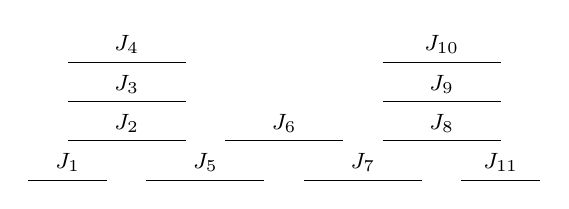
\begin{tikzpicture}[scale=0.5]\footnotesize
    \draw (0,0) -- (2, 0) node[midway,auto] {\footnotesize $J_1$}; 
    \draw (1,1) -- (4, 1) node[midway,auto] {\footnotesize $J_{2}$};
    \draw (1,2) -- (4, 2) node[midway,auto] {\footnotesize $J_{3}$};
    \draw (1,3) -- (4, 3) node[midway,auto] {\footnotesize $J_{4}$};
    \draw (3,0) -- (6, 0) node[midway,auto] {\footnotesize $J_{5}$}; 
    \draw (5,1) -- (8, 1) node[midway,auto] {\footnotesize $J_{6}$};
    \draw (7,0) -- (10, 0) node[midway,auto] {\footnotesize $J_{7}$};
    \draw (9,1) -- (12 , 1) node[midway,auto] {\footnotesize $J_{8}$};
    \draw (9,2) -- (12 , 2) node[midway,auto] {\footnotesize $J_{9}$};
    \draw (9,3) -- (12 , 3) node[midway,auto] {\footnotesize $J_{10}$};
    \draw (11,0) -- (13, 0) node[midway,auto] {\footnotesize $J_{11}$};
  \end{tikzpicture}
}

\smallskip

The third rule chooses $J_6=[5,8]$ first, but the only correct solution
is \[S=\{J_1, J_5, J_7, J_{11}\} = \{[0,2], [3,6], [7,10], [11,13]\},\]
which does not contain $J_6$.

\paragraph{Exercises without solutions}

\exercise\label{greedy: exercise: activity selection}
What is a correct output for the \prob{Activity Selection} instance below?

\[I = \{[0, 4], [2, 6], [3, 8], [7, 11], [9, 13], [10, 14], [12, 15], [12, 16], [14, 18]\}.\]

\centerline{
  \begin{tikzpicture}[scale=0.5]\footnotesize
    \draw (0,0) -- (4, 0) node[midway,auto] {\footnotesize $J_1$}; 
    \draw (2,1) -- (6, 1) node[midway,auto] {\footnotesize $J_{2}$};
    \draw (3,2) -- (8, 2) node[midway,auto] {\footnotesize $J_{3}$};
    \draw (7,0) -- (11, 0) node[midway,auto] {\footnotesize $J_{4}$};
    \draw (9, 1) -- (13, 1) node[midway,auto] {\footnotesize $J_{5}$}; 
    \draw (10,2) -- (14, 2) node[midway,auto] {\footnotesize $J_{6}$};
    \draw (12,3) -- (15, 3) node[midway,auto] {\footnotesize $J_{7}$};
    \draw (12,0) -- (16 , 0) node[midway,auto] {\footnotesize $J_{8}$};
    \draw (14,1) -- (18 , 1) node[midway,auto] {\footnotesize $J_{9}$};
  \end{tikzpicture}
}

\paragraph{External exercises without solutions}
\begin{itemize}
\item \KT Chapter 4, Exercise 17.  \CLRS Chapter 16, Exercises in Section 16.1.
\item \JE Chapter 4, Exercises 1, 2, 3 (Covering by Intervals), 4 (Puncturing)
\end{itemize}

\subsection{External sources on \prob{Activity Selection}}

\begin{itemize}
\item \KT Section 4.1 and \KWSlides (``Interval Scheduling'')
\item  \CLRS Chapter 16, Section 16.1.  \JE Chapter 4, Section 4.2.
\end{itemize}

% This gives us the following iterative algorithm:

% 1. Assume (by sorting the jobs if necessary) that the jobs are ordered by increasing ending time.
% 2. Initialize A to the empty set.
% 3. For each job J_d, in order of increasing ending time, do:
% 4.   If J_d conflicts with any job in A, skip it.
% 5.   Otherwise, add it to A.
% 6. Return A.

% It follows from the "general claim" above that the algorithm maintains the desired invariant.  Does this mean the algorithm is correct?  Not quite.  We know the invariant holds at the end.  So, the solution A at termination is a subset of some optimal solution S*.  But is A in fact an _entire_ optimal solution?  

% Suppose for contradiction that A is a proper subset of S*.  Then there is at least one job, say J_d, that is in S* but not A.  The algorithm considered J_d in some iteration, and when it did, it did not add it (because it is not in A now).  So, that job must have a conflict with some job in A.  But A is a subset of S*, so that job also has a conflict with some job in S*.  This contradicts that S* is an independent set.  So we can conclude that A is not a proper subset of S*.  So it must equal S*.  So A is an optimal solution.


%%% Local Variables:
%%% mode: latex
%%% TeX-master: "greedy_algorithms"
%%% End:
